\documentclass[oneside]{book}
\usepackage[utf8]{inputenc}
\usepackage[margin=1in]{geometry}
\usepackage{enumitem}
\usepackage{mathtext}
\usepackage{amssymb}
\usepackage[misc]{ifsym}
\usepackage{lipsum}
\usepackage{cancel}
\usepackage{pgfplots}
\pgfplotsset{width=10cm,compat=1.9}
\usepackage{tikz}
\usetikzlibrary{positioning}
\usepackage{caption}

\newcommand{\repeatcaption}[2]{%
  \renewcommand{\thefigure}{\ref{#1}}%
  \captionsetup{list=no}%
  \caption{#2 (repeated from page \pageref{#1})}%
}

\newcommand*{\ts}{\textsuperscript}

% ------------------------------------------------------ %
% Set up header
\usepackage{fancyhdr}
\pagestyle{fancy}
\renewcommand{\sectionmark}[1]{\markright{ - #1}}
\renewcommand{\chaptermark}[1]{\markboth{#1}{}}
\fancyhf{}
\fancyhead[L]{\leftmark\rightmark}
\fancyhead[R]{Page \thepage}

\fancypagestyle{plain}{
    \fancyhf{}
    \rhead{Page \thepage}
}
% ------------------------------------------------------ %

\title{STATS 230 Course Notes}
\author{Joshua Allum}
\date{April 2017}

\begin{document}
\maketitle
\tableofcontents

\chapter{Introduction}
\section{Defining Probability}
% ---------------------------------------------- %
% Classical Definition
\subsection*{The Classical Definition}
The probability of an event is
\[  
    \frac{\text{the number of ways the event may occur}}{\text{the total number of possible outcomes}}
\]
provided all outcomes are equally likely.
\begin{example}
The probability of a fair dice landing on 3 is 1/6 because there is one way in which the dice may land on 3 and 6 total possible outcomes of faces the dice may land on. The sample space of the experiment, $\sS$, is $\{1,2,3,4,5,6\}$ and the event occurs in only one of these six outcomes.
\end{example}
\begin{info}
The main limitation of this definition is that it demands that the outcomes of a sample space are equally likely. This is a problem since a definition of ``likelyhood'' (probability) is needed to include this postulate in a definition of probability itself.
\end{info}
% ---------------------------------------------- %
% Relative Frequency Definition
\subsection*{The Relative Frequency Definition}
The probability of an event is the limiting proportion of times that an event occurs in a large number of repetitions of an experiment.
\begin{example}
The probability of a fair dice landing on 3 is 1/6 because after a very large series of repetitions (ideally infinite) of rolling the dice, the fraction of times the face with 3 is rolled tends to 1/6.
\end{example}
\begin{info}
The main limitation of this definition is that we can never repeat a process indefinitely so we can never truly know the probability of an event from this definition. Additionally, in some cases we cannot even obtain a long series of repetitions of processes to produce an estimate due to restrictions on cost, time, etc.
\end{info}
% ---------------------------------------------- %
% Subjective Definition
\subsection*{The Subjective Definition}
The probability of an event occurring is a measure of how sure the person making the statement is that the event will occur.
\begin{example}
The probability that a football team will win their next match can be predicted by experts who regard all the data of past matches and current situations to provide a subjective probability.
\end{example}
\begin{info}
This definition is irrational and leads to many people having different probabilities for the same events, with no clear ``right'' answer. Thus, by this definition, probability is not an objective science.
\end{info}

% ---------------------------------------------- %
% Probability Model
\subsection*{Probability Model}
To avoid many of the limitation of the definitions of probability, we can instead treat probability as a mathematical system defined by a set of axioms. Thus, we can ignore the numerical values of probabilities until we consider a specific application. The model is defined as follows
\begin{itemize}
    \item A sample space of all possible outcomes of a random experiment is defined.
    \item A set of events, to which we may assign probabilities, is defined.
    \item A mechanism for assigning probabilities to events is specified.
\end{itemize}
\chapter{Mathematical Probability Models}
\section{Sample Spaces}
A sample space,~\sS, is a set of distinct outcomes for an experiment or process, with the property that in a single trial, one~and only~one of these outcomes occurs. The outcomes that make up a sample space are called sample points or simply points.
\begin{example}
The sample space for a roll of a six-sided die is
\[
    \{a_1,a_2,a_3,a_4,a_5,a_6\}\hspace{5mm}\text{where $a_i$ is the event the top face is $i$}
\]
More simply we could define the sample space as
\[
    \{1,2,3,4,5,6\}
\]
\end{example}
\begin{info}
Note that a sample space of a probability model for a process is not necessarily unique. Often times, however, we try to chose sample points that are the smallest possible or ``indivisible''.
\end{info}
\begin{example}
If we define $E$ to be the event that the top face of a six-sided~die is even when rolled and $O$ to be the event the top-face is odd, then the sample space,~\sS, can be defined as
\[
    \{E,O\}
\]
This is the same process as Example 2.1.1 (rolling a six-sided die), so since the sample spaces differ, clearly, sample spaces are not unique. Moreover, if we are interested in the event that a 3 is rolled, this sample space is not suitable since it groups the event in question with other events.
\end{example}
A sample space can be either \textbf{discrete} or \textbf{non-discrete}. If a sample space is discrete, it consists of a finite or countably infinite number ``simple~events''. A countably infinite set is one that can be put into a one-to-one correspondence with the set of real numbers. For example, $\left\{1,\frac{1}{2},\frac{1}{3},\frac{1}{4},\ldots\right\}$ is countably infinite whereas $\{x|x\in\sR\}$ is not.
\subsection*{Simple Events}
An event in a discrete sample space is a subset of the sample space, i.e., $A \subset \sS$. If the event is indivisible, so as to only contain one point, we call it a simple event, otherwise it is a compound event.
\begin{example}
A simple event for a roll of a six-sided die is $A = \{a_1\}$ where $a_i$ is the event the top face is i. A compound event is $E = \{a_2,a_4,a_6\}$.
\end{example}

\section{Assigning Probabilities}
Let $\sS = \{a_1,a_2,a_3,\ldots\}$ be a discrete sample space. We assign probabilities, $P(a_i),\for i = 1,2,3,\ldots$ to each sample point $a_i$ such that the following two conditions hold
\begin{itemize}
    \item $0 \leq P(a_i) \leq 1$
    \item $\sum\limits_{\all i} P(a_i) = 1$
\end{itemize}
The set of probabilities $\{P(a_i)|i = 1,2,3,\ldots\}$ is called a \textbf{probability distribution} on \sS.
\chapter{Counting Techniques}
\section{Counting Arguments}
If we have a sample space, \sS, of some experiment that has a \textbf{uniform distribution} (all sample points are equally likely), then we can calculate the probability of a compound event $A$ as the number of sample points in $A$ divided by the total number of sample points.
\[
    P(A) = \frac{k}{n}
\]
where $k$ is the number of sample points in $A$ and $n$ is the total number of sample points in the sample space.
\subsection*{Addition Rule}
Consider we can perform process 1 in $p$ ways and process 2 in $q$ ways. Suppose we want to do process~1 \textbf{or} process~2 \textbf{but not both}, then there are $p + q$ ways to do so.
\begin{example}
Suppose a keyboard only has 26 letters and 20 special characters (!\%\#\$), there are 46 ways in which a typist may type a \textbf{single} character. (Process 1: typing a letter. Process 2: typing a special character).
\end{example}
\subsection*{Multiplication Rule}
Again, consider we can perform process~1 in $p$ ways and process~2 in $q$ ways. Suppose we want to do process~1 \textbf{and} process~2, then there are $p \times q$ ways to do so. This is because \textbf{for each way} of doing process~1 we can do process~2 in $q$ ways.
\begin{example}
Suppose the same typist with the same keyboard wants to type a single letter \textbf{and} a single special character. The typist can do so in 520 ways, since there are 26 ways to select the letter and \textbf{for each} possible letter selection there are 20 possible special character selections.
\end{example}
\begin{info}
Try to associate \textbf{OR} and \textbf{AND} with \textbf{addition} and \textbf{multiplication} respectively in your mind.
\end{info}
\begin{info}
 Often times, \textbf{OR}'s and \textbf{AND}'s are not explicit or obvious so you must re-word your problem to identify implicit \textbf{OR}'s and \textbf{AND}'s.
\end{info}
\begin{example}
A young boy gets to pick 2 toys from a store for his birthday. How many ways can he pick 2 toys if the store contains 12 toys? He may pick the same toy multiple times and picks the toys at random.
\tcblower
We can re-word this problem as follows: A young boy selects one of 12 toys \textbf{and} again, selects one of 12 toys. Thus there are $12 \times 12 = 144$ ways in which he can select 2 toys. Furthermore, we have that since selections are random, each selection is equally likely. So the probability that the boy selects any pair of toys is 1/144.
\end{example}
\begin{info}
In this case the boy was allowed to select the same toy more than once. This is often referred to as \textbf{with replacement}. The addition and multiplication rules are generally sufficient to find probability of processes with replacement but if processes occur without replacement solutions become more complex and other techniques are often used.
\end{info}
\begin{info}
The phrase \textbf{at random} or \textbf{uniformly}, indicates that each point in the sample space is equally likely.
\end{info}
\chapter{Probability Rules}
\section{General Rules}
Here are a few basic rules of probabilities. They should be relatively straightforward.
\begin{theorem}
For a sample space, \sS, the probability of a simple event in \sS~occurring is 1. That is
\[
    P(\sS) = 1
\]
\end{theorem}
\begin{proof}
\[
    P(\sS) = \sum_{a \in \sS} P(a) = \sum_{\all a} P(a)
\]
\end{proof}
\begin{theorem}
Any event $A$ in a sample space has a probability between 0 and 1 inclusive. That is
\[
    0 \leq P(A) \leq 1 \for\all A\subseteq\sS
\]
\end{theorem}
\begin{proof}
Note that $A$ is a subset of \sS, so
\[
    P(A) = \sum_{a \in A} P(a) \leq \sum_{a \in \sS} P(a) = 1
\]
Now, recall that $P(a) \geq 0$ for any sample point $a$ by our probability model. Thus, since $P(A)$ is the sum of non-negative real numbers, $P(A) \geq 0$. So we have
\[
    1 \leq P(A) \leq 1
\]
\end{proof}
\begin{theorem}
If $A$ and $B$ are two events such that $A \subseteq B$, that is all the sample points in $A$ are also in $B$, then 
\[
    P(A) \leq P(B)
\]
\end{theorem}
\begin{proof}
\[
    P(A) = \sum_{a \in A} P(a) \leq \sum_{a \in B} P(a) = P(B)
\]
\end{proof}

\chapter{Conditional Probability}
Often we need to calculate the probability of some event~$A$ occurring while knowing that some other event~$B$ has already occurred. We call this the conditional probability of $A$ \textbf{given} $B$ and denote it by $P(A \given B)$.
\par\smallskip
The conditional probability of event~$A$, given event~$B$, is
\[
    P(A \given B) = \frac{P(A \intersect B)}{P(B)}\for P(B) > 0
\]
\section{Theorems and Rules for Conditional Probability}
\begin{theorem}
For any two events~$A$ and~$B$ defined on the same sample space, with $P(A) > 0$ and $P(B) > 0$, events~$A$ and~$B$ are independent if and only if $P(A \given B) = P(A)$ or $P(B \given A) = P(B)$.
\end{theorem}
\begin{proof}
\begin{align*}
    P(A \given B) &= \frac{P(A \intersect B)}{P(B)} \\
    \ifo 
    P(A \intersect B) &= P(A \given B)P(B)
\end{align*}
and by definition of independence,~$A$ and~$B$ are independent if and only if $P(A \intersect B) = P(A)P(B)$ which is true if and only if $P(A \given B) = P(A)$. Without loss of generality we can swap events~$A$ and~$B$ and arrive at the conclusion.
\end{proof}
\subsection*{Product Rules}
\begin{theorem}
Let $A, B, C$ and~$D$ be events on a sample space, with $P(A), P(B), P(C), P(D) > 0$. We have
\begin{align*}
    P(A \intersect B) &= P(A)P(B \given A) \\
    P(A \intersect B \intersect C) &= P(A)P(B \given A)P(C \given A \intersect B) \\
    P(A \intersect B \intersect C \intersect D) &=
    P(A)P(B \given A)P(C \given A \intersect B)P(D \given A \intersect B \intersect C) \\
\end{align*}
and so on$\ldots$
\end{theorem}
\begin{proof}
The first statement come directly from the definition of conditional probability
\[
    P(A)P(B \given A) = P(A) \frac{P(A \intersect B)}{P(A)} = P(A \intersect B)
\]
For the second we have
\begin{align*}
    P(A)P(B \given A)P(C \given A \intersect B)
    &= P(A \intersect B)P(C \given A \intersect B)
    &\by{the first statement} \\
    &= P(A \intersect B) \frac{P(A \intersect B \intersect C)}{P(A \intersect B)}
    &\by{definition of conditional probability} \\
    &= P(A \intersect B \intersect C)
\end{align*}
and so on$\ldots$
\end{proof}
\subsection*{Law of Total Probability}
\begin{theorem}
Let $A_1, A_2, A_3,\ldots,A_k$ be mutually exclusive events on a sample space and let $B$ be an event on the same sample space. We have
\[
    P(B) = P(B \intersect A_1) + P(B \intersect A_2) + P(B \intersect A_3) + \cdots + P(B \intersect A_k)
    = \sum_{i = 1}^{k} P(A_i)P(B \given A_i)
\]
\end{theorem}
\begin{proof}
Note that the events $A_i \intersect B$ for $1 \leq i \leq k$ are all mutually exclusive events since $A_i$'s are mutually exclusive. Thus, the union of the $A_i \intersect B$'s is $B$, that is 
\[
    (A_1 \intersect B) \union (A_2 \intersect B) \union (A_3 \intersect B) \union \cdots \union (A_k \intersect B) = B
\]
So by Theorem 4.5.1, we have
\[
    P(B) = P(A_1 \intersect B) + P(A_2 \intersect B) + P(A_3 \intersect B) + \cdots + P(A_k \intersect B)
\]
and by Theorem 5.1.2 (Product Rule), we have
\[
    P(B) = P(A_1)P(B \given A_1) + P(A_2)P(B \given A_2) + P(A_3)P(B \given A_3) + \cdots + P(A_k)P(B \given A_k) = \sum_{i = 1}^{k} P(A_i)P(B \given A_i)
\]
as required.
\end{proof}
\subsection*{Bayes' Theorem}
\begin{theorem}
Let $A$ and~$B$ be events on a sample space, with $P(B) > 0$. We have
\[
    P(A \given B) = \frac{P(B \given A)P(A)}{P(B)}
    = \frac{P(B \given A)P(A)}{P(B \given \comp{A})P(\comp{A}) + P(B \given A)P(A)}
\]
\end{theorem}
\begin{proof}
\begin{align*}
    P(A \given B)
    &= \frac{P(A \intersect B)}{P(B)} 
    = \frac{P(B \given A)P(A)}{P(B)}\by{Theorem 4.7.2 (Product Rule)} \\
    &= \frac{P(B \given A)P(A)}{P(A \intersect B) + P(\comp{A} \intersect B)}
    \by{Theorem 4.7.3 (Law of Total Probability)} \\
    &= \frac{P(B \given A)P(A)}{P(B \given \comp{A})P(\comp{A}) + P(B \given A)P(A)}\by{Theorem 4.7.2 (Product Rule)}
\end{align*}
\end{proof}
\begin{info}
Bayes' Theorem allows us to find the conditional probability of some event~$A$ given~$B$, in terms of the probability of~$B$ given~$A$. It allows us calculate conditional probabilities using the reversed order of conditioning.
\end{info}
\section{Tree Diagrams}
Tree diagrams are a technique that we can use to keep track of conditional probabilities. We start from a single node and draw new branches to separate nodes for each event. Each node represents the event occurring. On each branch we write the probability of event it leads to occurring. To find the probability of any node we multiply the probabilities of the branches leading to the node.
\begin{figure}[htp]
\centering
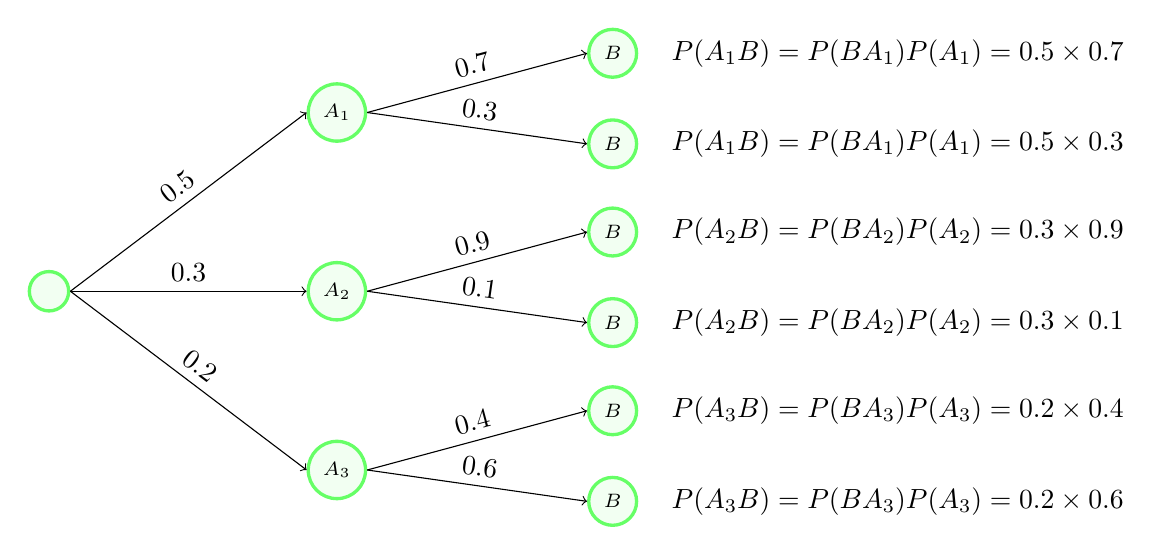
\begin{tikzpicture}[
roundnode/.style={circle, draw=green!60, fill=green!5, very thick, minimum size=5mm},
]
%Nodes
\node[roundnode]        (root)                              {};
\node[roundnode]        (A2)        [right=3cm of root]                 {$\scriptstyle A_2$};
\node[roundnode]        (A1)        [above=1.5cm of A2]                 {$\scriptstyle A_1$};
\node[roundnode]        (A3)        [below=1.5cm of A2]                 {$\scriptstyle A_3$};
\node[roundnode]        (A1B)       [above right=0.25cm and 3cm of A1]   {$\scriptstyle B$};
\node[roundnode]        (A1compB)   [below=0.5cm of A1B]                {$\scriptstyle\comp{B}$};
\node[roundnode]        (A2B)       [above right=0.25cm and 3cm of A2]   {$\scriptstyle B$};
\node[roundnode]        (A2compB)   [below=0.5cm of A2B]                {$\scriptstyle\comp{B}$};
\node[roundnode]        (A3B)       [above right=0.25cm and 3cm of A3]   {$\scriptstyle B$};
\node[roundnode]        (A3compB)   [below=0.5cm of A3B]                {$\scriptstyle\comp{B}$};
 
%Lines
\draw[->] (root.east) -- (A1.west) node[midway, sloped, above] {0.5};
\draw[->] (root.east) -- (A2.west) node[midway, sloped, above] {0.3};
\draw[->] (root.east) -- (A3.west) node[midway, sloped, above] {0.2};
\draw[->] (A1.east) -- (A1B.west) node[midway, sloped, above] {0.7};
\draw[->] (A1.east) -- (A1compB.west) node[midway, sloped, above] {0.3};
\draw[->] (A2.east) -- (A2B.west) node[midway, sloped, above] {0.9};
\draw[->] (A2.east) -- (A2compB.west) node[midway, sloped, above] {0.1};
\draw[->] (A3.east) -- (A3B.west) node[midway, sloped, above] {0.4};
\draw[->] (A3.east) -- (A3compB.west) node[midway, sloped, above] {0.6};

%Probabilities
\node [right=3mm of A1B]
    {$P(A_1 \intersect B) = P(B \given A_1)P(A_1) = 0.5 \times 0.7$};
\node [right=3mm of A1compB]
    {$P(A_1 \intersect \comp{B}) = P(\comp{B} \given A_1)P(A_1) = 0.5 \times 0.3$};
\node [right=3mm of A2B]
    {$P(A_2 \intersect B) = P(B \given A_2)P(A_2) = 0.3 \times 0.9$};
\node [right=3mm of A2compB]
    {$P(A_2 \intersect \comp{B}) = P(\comp{B} \given A_2)P(A_2) = 0.3 \times 0.1$};
\node [right=3mm of A3B]
    {$P(A_3 \intersect B) = P(B \given A_3)P(A_3) = 0.2 \times 0.4$};
\node [right=3mm of A3compB]
    {$P(A_3 \intersect \comp{B}) = P(\comp{B} \given A_3)P(A_3) = 0.2 \times 0.6$};
\end{tikzpicture}
\caption{Tree diagram} \label{fig:Tree diagram}
\end{figure}
\begin{info}
The probability of all the the branches leading outward from each node must sum to~ 1 since at least one outcome must occur.
\end{info}

\chapter{Useful Sums and Series}
This chapter includes a few useful sums and series that show up in the following chapters.
\section{Geometric Series}
\[
    \sum_{i = 0}^{n-1} r^i = 1 + r + r^2 + \cdots + r^{n-1} = \frac{1-r^n}{1-r}
\]
For $\abs{r} < 1$, we have
\[
    \sum_{i = 0}^{\infty} r^i = 1 + r + r^2 + \cdots = \frac{1}{1-r}
\]
\begin{info}
Other identities can be obtained from this one by differentiation. For example we have
\[
    \deriv r\sum_{i = 0}^{\infty} r^i = \sum_{i = 0}^{\infty} ir^{i-1} = \deriv r\,\frac{1}{1-r} = \frac{1}{(1-r)^2}
\]
\end{info}
\section{Binomial Theorem}
The binomial theorem describes the algebraic expansion of powers of a polynomial.
\[
    (1 + t)^n = 1 + \binom{n}{1}t^1 + \binom{n}{2}t^2 + \cdots + \binom{n}{n}t^n = \sum_{x = 0}^{n} \binom{n}{x} t^x
\]
for any positive integer $n$ and real number $t$.
\par\smallskip
A more general form of this theorem that holds even when $n$ is not a positive~integer is
\[
    (1 + t)^n = \sum_{x = 0}^{\infty} \binom{n}{x} t^x,\:\for \abs{t} < 1
\]
\begin{info}
It is an important skill to be able to recognize if an infinite, or otherwise, polynomial with binomial coefficients can be reduced to a simple polynomial raised to a power.
\end{info}
\section{Multinomial Theorem}
The multinomial theorem is a generalization of the binomial theorem. It describes the algebraic expansion of powers of a sum in terms of powers of the terms in the sum.
\[
    (x_1 + x_2 + \cdots + x_m)^n = \sum_{k_1 + k_2 + \cdots + k_m = n} \binom{n}{k_1,k_2,\ldots,k_m} \prod_{t = 1}^{m} x_t^{k_t}
\]
Another common form in which this theorem may be represented is
\[
    (x_1 + x_2 + \cdots + x_m)^n 
    = \sum_{k_1 + k_2 + \cdots + k_m = n} \frac{1}{k_1!\,k_2!\cdots k_m!}(x_1^{k_1}x_2^{k_2}\cdots x_m^{k_m})
\]
\begin{info}
The summation is over all non-negative integers, $k_1,k_2,\ldots,k_m$ such that $k_1 + k_2 + \cdots + k_m = n$
\end{info}
\section{Hypergeometric Identitiy}
\[
    \sum_{x = 0}^{\infty} \binom{a}{x} \binom{b}{n-x} = \binom{a + b}{n}
\]
\begin{proof}
We begin with the equality
\[
    (1 + y)^{a + b} = (1 + y)^a \times (1 + y)^b
\]
Now by Binomial Theorem we have
\[
    \sum_{k = 0}^{a + b} \binom{a + b}{k} y^k = \sum_{i = 0}^{a} \binom{a}{i} y^i \times \sum_{j = 0}^{b} \binom{b}{j} y^j
\]
Consider the coefficient of $y^k$ on the right hand side. It is the sum of all the binomial terms such that $i + j = k$. Thus, the coefficient of $y^k$ on the right hand side is
\[
    \sum_{i = 0}^{\min\{\, a,k \,\}} \binom{a}{i} \binom{b}{k-i}
\]
and since when $i > a$ or $i > k$ the term is 0 we can increase the sum to infinity. Thus, since the coefficient on the right hand side is equal to that on the left hand side we have
\[
    \binom{a + b}{k} = \sum_{i = 0}^{\infty} \binom{a}{i} \binom{b}{k-i}
\]
\end{proof}
\begin{info}
When $x$ becomes significantly large, the terms of the summation become 0 since 
\[
    \binom{n}{x} = \binom{n}{n-x} = 0,\:\for x > n
\]
\end{info}

\chapter{Discrete Random Variables and Probability Functions}
\section{Random Variables}
\lipsum[2]
\section{Probability Function}
\lipsum[1]
\section{Cumulative Distribution Function}
\lipsum[3]

\chapter{Discrete Distributions}
As we briefly mentioned in the previous chapter, \textbf{probability distributions} are the set of pairs~$(x,f(x))$ for all possible outcomes~$x$ of a random variable~$X$. Many probability distributions appear commonly on \rv's of similar ``real-life'' processes. In this chapter we define a few of these common distributions on discrete random variables, when they occur and how to use them to calculate probabilities.
\begin{info}
It is important to understand distributions early-on. Distributions, probability functions and cumulative distribution functions are defined on random variables \textbf{not} experiments/processes or sample spaces.
\end{info}

\section{Uniform Distribution}
Suppose $X$ can take a finite set of consecutive values with each of the values being equally likely. That is $\range{X} = \{\, a,a+1,a+2,\ldots,b \,\}$ with each of $a,a+1,a+2,\ldots,b$ being equally likely. Then $X$ has a discrete uniform distribution and we denote it \\
$X \dist \duni$
\[
    f(x) = P(X = x) = \left\{
    \begin{array}{c@{\hspace{1em}}l}
        \displaystyle\frac{1}{b - a + 1} & \for\all x\in\range{X} \\[1em]
         0 & \ow 
    \end{array}\right.
\]
\begin{theory}{Derivation of Probability Function}
The probability of each value of the \rv~is easy to calculate since they are all equal and must add up to 1. Therefore, $k \times P(X = a) = 1$ where $k$ is the number of possible values of $X$. The number of possible values of $X$ is $b - (a - 1) = b - a + 1$ since $\range{X}$ is between $a$ and $b$ inclusive.
\end{theory}
\begin{info}
Another way to define the probability of each value of a random variable with this sample space is 
\[
\frac{1}{\text{Number of possible values in $\range{X}$}}
\]
\end{info}
\section{Hypergeometric Distribution}
Suppose we have a collections of $N$ objects which can be classified into two different types, successes and failures. There are $r$ successes and $N -r$ failures. We pick $n$ objects at random without replacement, and let the random variable $X$ be the number of successes obtained. $X$ has a hypergeometric distribution and we denote it \\
$X\dist\hype$
\[
    f(x) = P(X = x) =
    \frac{\displaystyle\binom{r}{x}\binom{N-r}{n-x}}{\displaystyle\binom{N}{n}},\:\for x\leq\min(r,n)
\]
\begin{theory}{Derivation of Probability Function}
We will use the counting techniques we previously learnt to calculate the probability function. We note that there are $\binom{N}{n}$ ways to select $n$ objects from the total of $N$ so the sample space contains $\binom{N}{n}$~points. Now the number of ways of choosing $x$ successes from the total of $r$ is $\binom{r}{x}$ \textbf{and independently} the number of ways to choose the remainder of objects, $n-x$, from the total remaining objects, $N - r$, is $\binom{N - r}{n - x}$. Thus the probability of~$X = x$ by the multiplication rule is the product of those expressions divided by the number of points in the sample space, $\frac{\binom{r}{x}\binom{N-r}{n-x}}{\binom{N}{n}}$.
\end{theory}
\begin{info}
It is important to understand that the terms ``successes'' and ``failures'' are simply placeholder that represent a type of outcome and its complement. They could be replaced by ``wins'' and ``losses'', ``whites'' and ``colors'', or any other titles that are distinct groups with a union that spans the whole sample space.
\end{info}
\begin{info}
    This is used when we know how many items (n) are chosen at random from a set with two different types and we know the amount of each type in the set.
\end{info}
\begin{example}
    There is a basket with 11 fruit, 9 apples and 2 oranges. 4 fruit are picked at random from the basket. Let random variable $X$ be the number of apples selected. Find $f(x)=P(X=x)$. Then find $f(3)$. \\
    $X\dist\hype$. $N=11,n=4,r=9$.
    \[f(x)=P(X=x)=\displaystyle\frac{\displaystyle\binom{9}{x}\binom{2}{4-x}}{\displaystyle\binom{11}{4}}\for x\leq4\]
    Hence \[f(7)=P(X=7)=\displaystyle\frac{\displaystyle\binom{9}{3}\binom{2}{1}}{\displaystyle\binom{11}{4}}\approx0.509\]
\end{example}
\begin{example}
    15 cards are drawn from a deck of 52 at random. Let $X$ be the number of red cards drawn. Find $f(x)=P(X=x)$. Then find $f(7)$. \\
    $X\dist\hype$. $N=52,n=15,r=26$.
    \[f(x)=P(X=x)=\displaystyle\frac{\displaystyle\binom{26}{x}\binom{26}{15-x}}{\displaystyle\binom{52}{15}}\for x\leq15\]
    Hence \[f(7)=P(X=7)=\displaystyle\frac{\displaystyle\binom{26}{7}\binom{26}{8}}{\displaystyle\binom{52}{15}}\approx0.229\]
\end{example}
\chapter{Mean and Variance}

% ------------------------------------------------------ %
\section{Summarizing Data on Random Variables}
Often times, listing out all of the outcomes of a sample is not a very helpful way of communicating the information obtained from the sample. A common, more helpful way to present the data of a sample is a \textbf{frequency distribution}. A frequency distribution gives the number of times each value of a random variable $X$ occurred.
\begin{center}
\begin{tabular}{ |c|c|c|c| } 
\hline
$X$ & Frequency Count & Frequency \\
\hline
1 & \StrokeTwo & 2 \\ 
2 & \StrokeFive\StrokeOne & 6 \\ 
3 & \StrokeFive & 5 \\
4 & \StrokeThree & 3 \\
\hline
\end{tabular}
\end{center}
We could also draw a \textbf{frequency histogram} of these frequencies.
\begin{center}
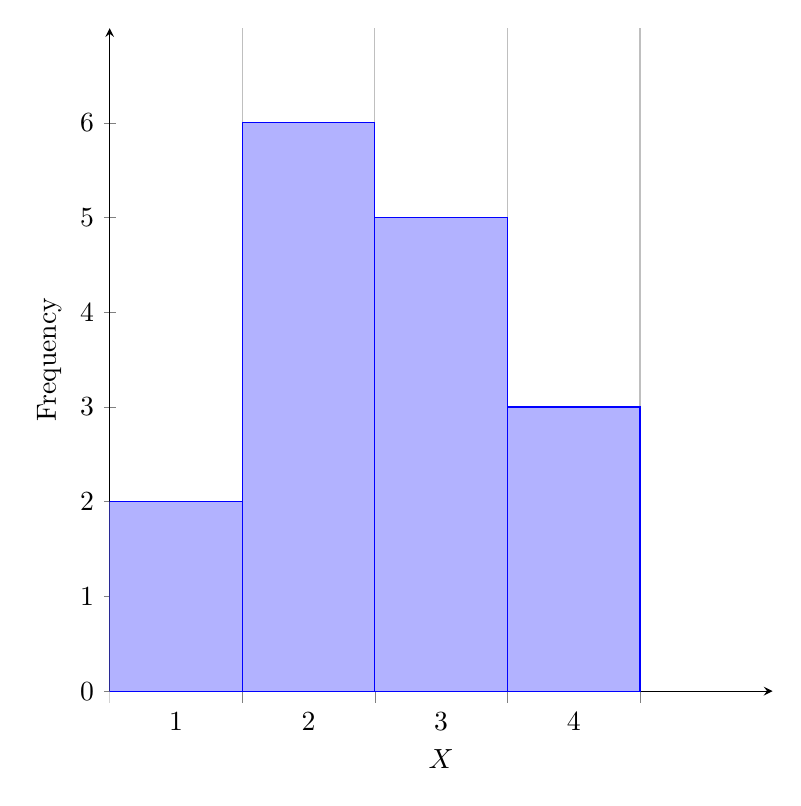
\begin{tikzpicture}
\begin{axis}[
	ylabel=Frequency,xlabel=$X$,
	axis lines=left,
	ymax=7,
	xmax=5,
	ybar interval=1,
	ytick = {0,...,6},
	width=10cm,height=10cm,
]
\addplot
	coordinates {(4,3) (3,5) (2,6) (1,2) (0,0)};
\end{axis}
\end{tikzpicture}
\end{center}
Frequency distributions are good summaries of data because they show the variability in the observed outcomes clearly. Another way to summarize results are single-number summaries such as the following:
\bigskip\par
The \textbf{mean} of a sample of outcomes is the average value of the outcomes. It is the sum of the outcomes divide by the total number of outcomes. The mean of $n$ outcomes, $x_1,\ldots,x_n$, for a random variable $X$ is
\[
    \sum_{i = 0}^{n} \frac{x_i}{n} = \frac{x_1,\ldots,x_n}{n}
\]
\bigskip\par
The \textbf{median} of a sample is an outcome such that half the outcomes are before it and half the outcomes are after it when the outcomes are arranged in numerical order.
\bigskip\par
The \textbf{mode} of a sample is the outcome that occurs most frequently. There can be multiple equal modes in a sample.
\bigskip\par
\begin{example}
A fisherman records the weight of each fish he catches for a week. These are his results. Each value represents the weight, in pounds, of a fish he caught.
\[
    \{\, 20,23,19,27,17,22,18,15,23,25,18,23,29 \,\}
\]
A frequency distribution of the sample above is
\begin{center}
\begin{tabular}{ |c|c|c|c| } 
\hline
$X$ & Frequency Count & Frequency \\
\hline
15 & \StrokeOne & 1 \\ 
17 & \StrokeOne & 1 \\ 
18 & \StrokeTwo & 2 \\ 
19 & \StrokeOne & 1 \\
20 & \StrokeOne & 1 \\
22 & \StrokeOne & 1 \\ 
23 & \StrokeThree & 3 \\ 
25 & \StrokeOne & 1 \\ 
27 & \StrokeOne & 1 \\
29 & \StrokeOne & 1 \\
\hline
\end{tabular}
\end{center}
And the following is a frequency histogram
\begin{center}
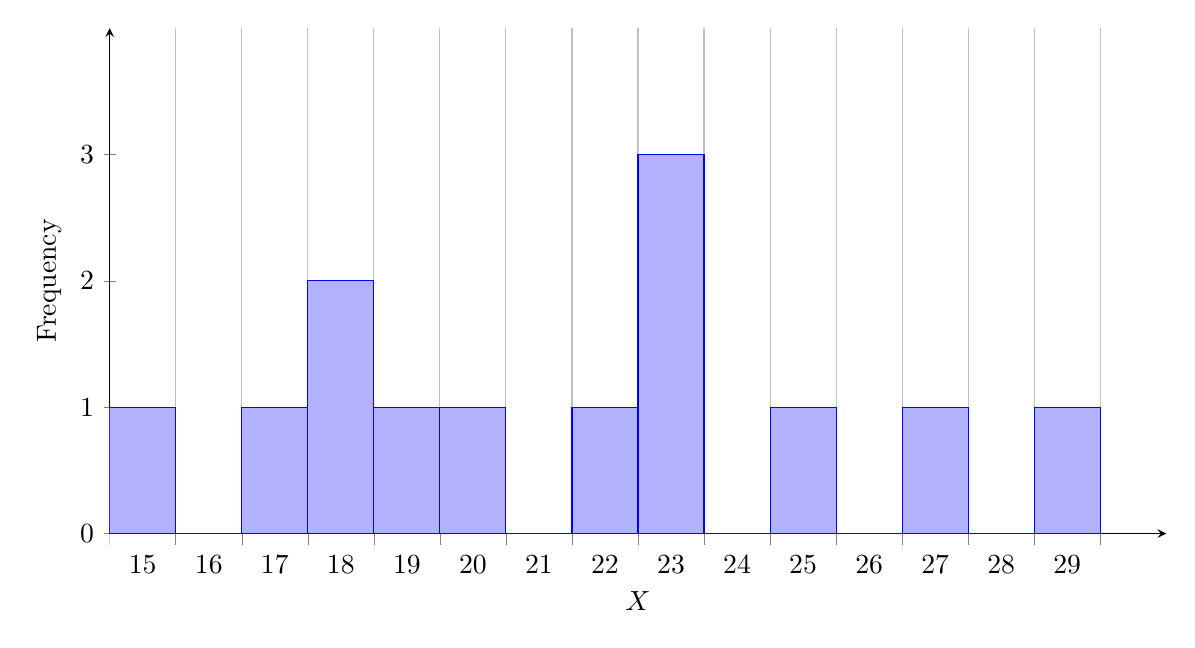
\begin{tikzpicture}
\begin{axis}[
	ylabel=Frequency,xlabel=$X$,
	axis lines=left,
	ymax=4,	
	xmin=14,
	xmax=30,
	ybar interval=1,
	ytick = {0,1,2,3},
	width=15cm,height=8cm,
]
\addplot
	coordinates {(29,1) (28,0) (27,1) (26,0) (25,1) (24,0) (23,3) (22,1) (21,0) (20,1) (19,1) (18,2) (17,1) (16,0) (15,1) (14,0)};
\end{axis}
\end{tikzpicture}
\end{center}
The mean weight of sample of fishes is
\[
    \frac{20+23+19+27+22+18+15+23+18+23+29}{13} = \frac{237}{13} \approx 18.231
\]
The median weight of the sample of fishes is found by rearranging the sample into numerical order and selecting the middle outcome. The median is 22.
\[
    15,18,18,19,20,\underuparrow{22},23,23,23,27,29
\]
The mode is the weight that occurs most frequently. It corresponds to tallest bar on the histogram. 23lbs occurs the most (3 times) so it is the median.
\end{example}

% ------------------------------------------------------ %
\section{Expected Value of a Random Variable}
The expected value of a random variable $X$ with a range of $A$ and a probability function $f(x)$, is given by
\[
    E(X) = \mean = \sum_{x \in A} xf(x)
\]
\begin{info}
Note that in order to calculate the expected value of a random variable $X$, we often need to know the distribution, and hence the probability function, of $X$.
\end{info}
\begin{theory}{Derivation of the Expected Value}
Suppose we have a frequency distribution of a random variable X, as shown below:
\begin{center}
\begin{tabular}{ |c|c|c|c| } 
\hline
$X$ & Frequency Count & Frequency \\
\hline
5 & \StrokeFive\StrokeFive & 10 \\ 
10 & \StrokeFive\StrokeTwo & 7 \\ 
25 & \StrokeFive\StrokeFive\StrokeThree & 13 \\
100 & \StrokeFour & 4 \\
200 & \StrokeTwo & 1 \\ 
\hline
\end{tabular}
\end{center}
As we learnt in the previous section, we can calculate the mean as
\begin{align*}
    &\frac{(5\times10) + (10\times2) + (25\times13) + (100\times4) + (200\times1)}{30} \\
    &= (5)\left(\frac{10}{30}\right) + (10)\left(\frac{7}{30}\right) + (25)\left(\frac{13}{30}\right) + (100)\left(\frac{4}{30}\right) + (200)\left(\frac{1}{30}\right) \\
    \text{($A$ is the range  of $X$) }
    &=\sum_{x \in A} x \times \text{the fraction of times $x$ occurs}
\end{align*}
Now suppose we know the probability function of $X$ is as follows
\renewcommand{\arraystretch}{1.5}
\begin{center}
\begin{tabular}{ c|c c c c c } 
$x$ & 5 & 10 & 25 & 100 & 200 \\
\hline
$f(x)$ & $\frac{1}{3}$ & $\frac{7}{30}$ & $\frac{13}{30}$ & $\frac{2}{15}$ & $\frac{1}{30}$ \\
\end{tabular}
\end{center}
Using the relative frequency definition of probability, we know that if we observed a very large number of outcomes, the fraction of times $X=x$ occurs (relative frequency of $x$) is $f(x)$. \\ Thus, \textit{in theory}, we would expect the mean of a sample of infinitely many outcomes to be
\[
    (5)\left(\frac{1}{3}\right) + (10)\left(\frac{7}{30}\right) + (25)\left(\frac{13}{30}\right) + (100)\left(\frac{2}{15}\right) + (200)\left(\frac{1}{30}\right) \approx 33.167
\]
This theoretical mean is denoted by $\mu$ or $E(X)$, and is known as the expected value of $X$.
\end{theory}
\begin{example}
A slots machine in a casino costs \$5 to play. It has probabilities of 0.5 to pay out \$2, 0.2 to pay out \$5, a 0.1 to pay out \$10 and otherwise does not pay out anything. Let the random variable $X$ be the amount of money (in dollars) the machine pays out in one play, and $Y$ be the amount of money won or lost in one play. Find $E(X)$ and $E(Y)$.
\[
    E(X) = (0)(0.2) + (2)(0.5) + (5)(0.2) + (10)(0.1) = 3
\]
\[
    E(Y) = (-5)(0.2) + (-3)(0.5) + (0)(0.2) + (5)(0.1) = -2
\]
Note that $E(Y) = E(X - 5) = E(X) - 5$
\end{example}

\begin{example}
A nightclub lets groups of up to 6 people enter at reduced fees. A randomly selected group in the nightclub's line has the following probabilities for its size and cost of entry:
\begin{center}
\begin{tabular}{ |c|c|c| } 
\hline
Size of Group (X) & Cost of Entry (Y) & Probability \\
\hline
1 & \$10 & 0.1 \\
2 & \$18 & 0.15 \\
3 & \$26 & 0.1 \\
4 & \$34 & 0.3 \\
5 & \$42 & 0.15 \\
6 & \$50 & 0.2 \\
\hline
\end{tabular}
\end{center}
1. Let $X$ be the size of a randomly selected group. Find $E(X)$.
\[
    E(X) = (0.1)(1) + (0.15)(2) + (0.1)(3) + (0.3)(4) + (0.15)(5) + (0.2)(6) = 3.85
\]
2. If the cost of entry of a group (Y) is $8 \times\text{the size of the group}+2$. Find the expected value of the cost of entry, in dollars, of a randomly selected group.
\[
    E(8X + 2)
    = E(Y) 
    = (0.1)(10) + (0.15)(18) + (0.1)(26) + (0.3)(34) + (0.15)(42) + (0.2)(50)
    = 32.8
\]
3. Show that the expected value of the cost of entry of a randomly selected group is $8 \times \text{the expected value of the size of the group} + 2$.
\[
    8E(X) + 2 = 8 \times 3.85 + 2 = 30.8 + 2 = 32.8 = E(8X + 2)
\]
\end{example}

\begin{theorem}
Let $X$ be a discrete random variable with a range of A, and probability function $f(x)$. The expected value of some function g(X) is given by
\[
    E\left[g(X)\right] = \sum_{x \in A} g(x)f(x)
\]
\end{theorem}
\begin{proof}
Let the random variable $Y = g(X)$ have a range of $B$ and a probability function $f_{\scriptscriptstyle Y}(y) = P(Y = y)$.
\[
    E[g(X)] = E(Y) = \sum_{y \in B} yf_{\scriptscriptstyle Y}(y)
\]
Now, let $C_y$ be $\{\, x \ssep g(x) = y \,\}$, that is the set of all values of $x$ such that $g(X)$ is $y$. So
\[
    f_{\scriptscriptstyle Y}(y) = P[g(X) = y]=\sum_{x \in C_y} f(x)
\]
That is, the probability that $Y = y$ is the sum of the probabilities that $X = x$ such that $g(x) = y$. \\
Now, we have
\begin{align*}
    E[g(X)] &= \sum_{y \in B} yf_{\scriptscriptstyle Y}(y) 
             = \sum_{y \in B} y\sum_{x \in C_y}  f(x) 
             = \sum_{y \in B}  \sum_{x \in C_y} yf(x) \\
            &= \sum_{y \in B}  \sum_{x \in C_y}  g(x)f(x)&
\end{align*}
Note that the inner summation is for all $x$ such that $g(x) = y$ and the outer is for all $y$. Thus the equation is the sum for all $x$. So
\[
    E[g(X)] = \sum_{y \in B} \sum_{x \in C_y} g(x)f(x) 
            = \sum_{x \in A} g(x)f(x)
\]
where $A$ is the range of X, as required.
\end{proof}

\subsection*{Linear Properties of Expected Value}
\begin{theorem}
For constants $a,b$ and $c$,
\[
    E[ag_1(X) + bg_2(X) + c] = aE[g_1(X)] + bE[g_2(X)] + c
\]
\end{theorem}
\begin{proof}
\begin{align*}
    E[aE[g_1(X)] + bE[g_2(X)]+c]
    &= \sum_{\all x} [ag_1(x)+bg_2(x)+c]f(x) \\
    &= \sum_{\all x} [ag_1(x)f(x)+bg_2(x)f(x)+cf(x)] \\
    &= \sum_{\all x}ag_1(x)f(x)+\sum_{\all x}bg_2(x)f(x)+\sum_{\all x}cf(x) \\
    &= a\sum_{\all x}g_1(x)f(x)+b\sum_{\all x}g_2(x)f(x)+c\sum_{\all x}f(x) \\
    \left(\text{recall }\sum_{\all x}f(x) = 1\right) \hspace{1cm}
    &= aE[g_1(X)] + b[g_2(X)] + c
\end{align*}
\end{proof}
% ====================================================== %

\section{Variance of a Random Variable}
The variance of a random variable~$X$ is given by
\[
    \var(X) = \stddev^2 = E\left[(X - \mean)^2\right]
\]
where $\stddev$ is the standard deviation of $X$. It is the average squared deviation of a random variable from its mean. It measures how far out from the mean the values of a random variable are spread.
\smallskip\par
The definition and formula above is useful in understanding the variance's importance but it can be difficult to use to actually calculate the variance. Here are a few other useful formulas for calculating the variance of a random variable:
\begin{align}
    \var(X) &= E(X^2) - [E(X)]^2 = E(X^2) - \mean^2 \label{eqn: variance alt formula}\\
    \var(X) &= E[X(X-1)] + E(X) - [E(X)]^2 = E[X(X-1)] + \mean - \mean^2
\end{align}
\begin{theory}{Derivation of Alternative Formulas}
\begin{align*}
    \var(X) = \stddev^2 
    &= E\left[(X - \mean)^2\right] \\
    &= E\left[X^2 -2X\mean + \mean^2\right] \\
    &= E(X^2) - 2\mean E(X) + \mean^2,\:\text{(by linear property since $\mean$ is a constant)} \\
    &= E(X^2) - 2\mean^2 + \mean^2,\:\text{(since $E(X) = \mean$)} \\
    &= E(X^2) - \mean^2
\end{align*}
Now note that $X^2 = X(X-1) + X$, so we have
\begin{align*}
    \var(X) = \stddev^2
    &= E[X(X-1) + X]  - \mean^2 \\
    &= E[X(X-1)] + E(X) -\mean^2 \\
    &= E[X(X-1)] + \mean -\mean^2
\end{align*}
\end{theory}
\subsection*{Properties of Variance}
\begin{theorem}
For constants $a$ and~$b$,
\[
    \var[aX + b] = a^2\var(X)
\]
\end{theorem}
\begin{proof}
\begin{align*}
    \var[aX + b]
    &= E\bigl[(aX + b)^2\bigr] - \bigl[E(aX + b)\bigr]^2,\hspace{12pt}\text{\big (by equation \eqref{eqn: variance alt formula}\big)} \\
    &= E\bigl[a^2 X^2 + 2abX + b^2\bigr] - \bigl[aE(X) + b\bigr]^2 \\
    &= a^2 E(X^2) + 2ab E(X) + b^2 - a^2[E(X)]^2 - 2abE(X) - b^2 \\
    &= a^2 \left(E(X^2) - [E(X)]^2\right) \\
    &= a^2 \var(X)
\end{align*}
\end{proof}
\subsection{Standard Deviation of a Random Variable}
The standard deviation of a random variable~$X$ is defined as
\[
    \stddev = \sqrt{\mathstrut\var X} 
    = \sqrt{\mathstrut E\bigl[(X - \mean)^2\bigr]}
\]
It is another measure used to quantify the variability of a random variable.
\begin{info}
A useful property of the standard deviation is that it is expressed in the same units as the random variable, unlike the variance.
\end{info}
\end{document}
